\documentclass{article}
\usepackage{graphicx} % Required for inserting images
\usepackage{minted}
\newcommand{\pr}{\mathop{\mathrm{Pr}}}
\newcommand{\ex}{\mathop{\mathrm{E}}}

\title{Simulation Methods in Statistics}
\author{Alex Zhou}
\date{April 2019}

\begin{document}

\maketitle

\section{Introduction}

Let \(X\) be a random variable and let \(F(x) = \pr(X \leq x)\) be a distribution function on \(X\). We assume for simplicity that \(F(x)\) is continuous and strictly increasing. Define \(U = F(X)\) which is a random variable with values in \([0,1]\). Then
\begin{eqnarray*}
    \pr(U \leq u) & = & \pr(F(X) \leq u) \\
                 & = & \pr(X \leq F^{-1}(u)) \\
                 & = & F(F^{-1}(u)) = u
\end{eqnarray*}
for \(u \in [0,1]\), hence has a uniform (rectangular) distribution on \([0,1]\) which we write as \(U \sim \mathop{\mathrm{Unif}}[0,1]\). Conversely, given \(U \sim \mathop{\mathrm{Unif}}[0,1] \), if we define \(X = F^{-1}(U)\), then \(X\) has distribution function \(F\). We can use this to generate \(X_1, \dots, X_n\) random variables from a given distribution function \(F(x)\).

\section{Exponential Distribution}

Take \(F(x) = 1 - e^{-\theta x}\), which corresponds to an exponential distribution with rate \(\theta\), mean \(\theta^{-1}\) and probability density \(f(x \mid \theta) = \theta e^{-\theta x}\), for \(x \geq 0\). Recall that the median is defined to be a number \(m\) such that
\[ \int_0^m f(x \mid \theta) \,dx = \frac{1}{2}. \]
For our exponential distributions, this evaluates to
\[ \int_0^m \theta e^{-\theta x} \,dx = [-e^{-\theta x}]^m_{x=0} = 1 - e^{-m\theta} = \frac{1}{2}, \]
which solves for \(\theta = \frac{\log 2}{m}\). Indexing the probability distribution function by the median instead, get
\[ g(x \mid m)= f(x \mid \theta(m)) = \frac{\log2}{m}\exp\left(-\frac{\log2}{m}x\right). \]
We sample \((u_1,\dots,u_n)\) from \(\mathop{\mathrm{Unif}}[0,1]\) and compute \(x_i\) defined by \(u_i = 1 - e^{-\theta_0 x_i}\) which yields \((x_1,\dots,x_n)\) sampled from \(f(x \mid \theta_0)\). 

\begin{minted}[autogobble, linenos]{python}
    def exp_sample(n, theta):
        u = np.random.uniform(0, 1, n)
        x = - (1 / theta) * np.log(1 - u)
        return x

    def log_likelihood(m, x):
        n = len(x)
        log2 = np.log(2)
        return n * np.log(log2) - n * np.log(m) - (log2 / m) * np.sum(x)
\end{minted}

The log-likelihood function is
\begin{eqnarray*}
    \ell_n(m) & = & \log\prod_{i=1}^n g(x_i \mid m) \\
              & = & \log\prod_{1=1}^n \frac{\log2}{m}\exp\left(-\frac{\log2}{m}x_i\right) \\
              & = & \sum_{i=1}^n\left(\log(\log2) - \log m - \frac{\log 2}{m}x_i \right) \\
              & = & n\log(\log 2) - n\log m - \frac{\log2}{m} \sum_{i=1}^n x_i.
\end{eqnarray*}
To minimise the log-likelihood, we take the derivative with respect to \(m\) and equate to \(0\),
\[ -\frac{n}{m} + \frac{\log 2}{m^2}\sum_{i=1}^n x_i = 0, \]
which yields the minimiser \(\hat{m}_n\) satisfying
\[ \hat{m}_n = (\log 2)\frac{\sum_{i=1}^n x_i}{n}. \]
By the law of large numbers this converges to the true median as \(n \to \infty\).

Set \(\theta_0 = 1.2\). We plot \(\ell_n(m)\) over \(m\) for sample sizes \(n = 6, 25, 50, 100\):
\begin{figure}
    \centering
    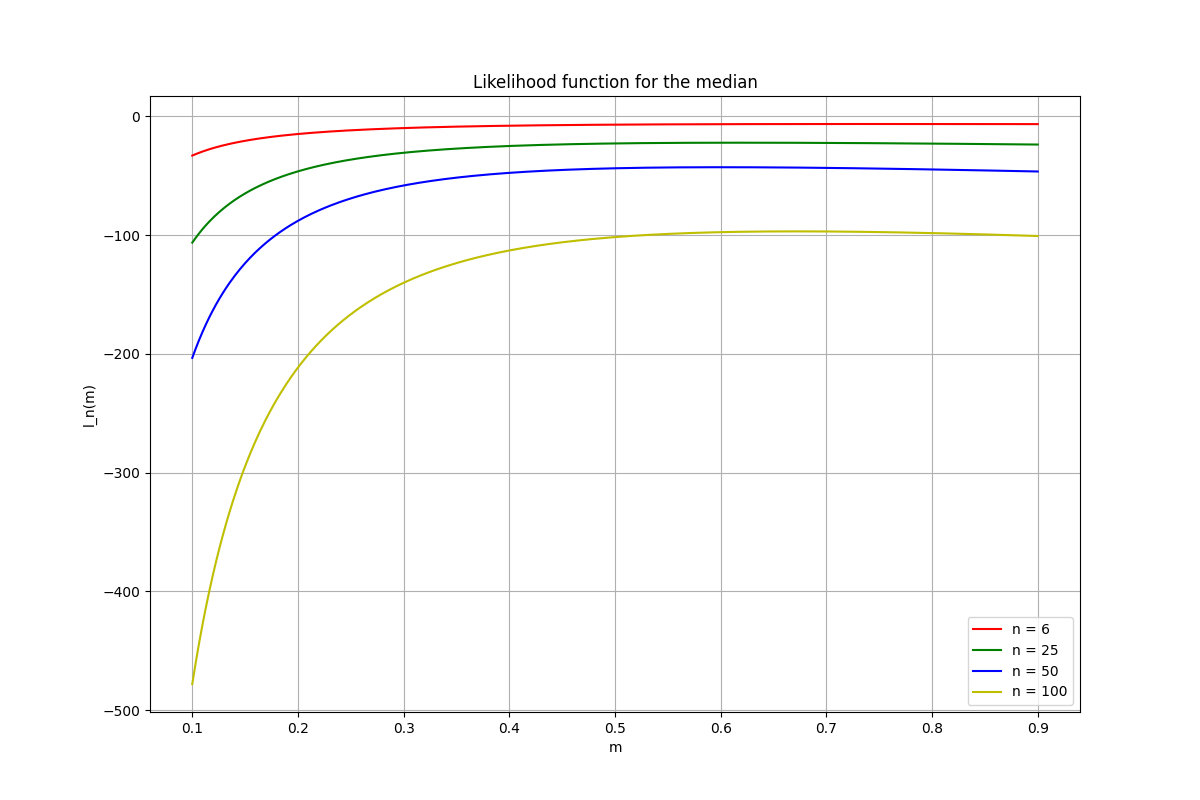
\includegraphics[width=1.0\linewidth]{images/exp_likelihood.png}
    \caption{A graph of the likelihood function of \(\mathop{\mathrm{Exp}}(1.2)\) for increasing samples.}
\end{figure}

The actual value for the median is \(\frac{\log 2}{\theta_0} = \frac{\log 2}{1.2} \approx 0.5776\). As we increase \(n\), we notice that the peak of the maximum likelihood gets closer and closer to this value. The likelihood function has expectation 
\[ n(\log(\log 2) - \log m - {\log 2}/{m\theta_0}),\]
so the graphs should have the shape of the sum of a logarithmic function and a reciprocal function, reflected. We note that the extreme values of the graphs move downwards as \(n\) increases. This reflects the fact that the likelihood of deviation from the median should become very rare as the sample size increases.

Let \(X, Y \sim \mathop{\mathrm{Exp}}(\theta)\) be independent exponentially distributed random variables. We aim to show that \(X+Y \sim \mathop{\Gamma}(2, \theta)\). First, we recall that the moment generating function of \(X\) is
\begin{eqnarray*}
    M_X(\lambda) & = & \ex[e^{\lambda X}] \\
                 & = & \int_0^\infty f(x \mid \theta) \,dx = \int_0^\infty \theta e^{x(\lambda - \theta)} \,dx \\
                 & = & \frac{\theta}{\lambda - \theta} [-e^{x(\lambda - \theta)}]_{x=0}^\infty = \frac{\theta}{\theta - \lambda},
\end{eqnarray*} 
whenever \(\lambda < \theta\). For \(X + Y\), we have
\begin{eqnarray*}
    M_{X+Y}(\lambda) & = & \ex[e^{\lambda(X+Y)}] = \ex[e^{\lambda X}e^{\lambda Y}] \\
                     & = & \ex[e^{\lambda X}] \ex[e^{\lambda Y}] \quad \mbox{by independence of X and Y,} \\
                     & = & \left(\frac{\theta}{\theta - \lambda}\right)^2 = \left(1 - \frac{\lambda}{\theta}\right)^2,
\end{eqnarray*}
for \(\lambda < \theta\). Uniqueness of moment generating functions means that \(X+Y \sim \mathop{\Gamma}(2, \theta)\), as desired. The probability density function of this distribution is given by \(f(x \mid \theta) = \theta^2 x e^{-\theta x}\) for \(x > 0\). Integrating to find the distribution function
\begin{eqnarray*}
    F(x) & = & \pr(X \leq x) \\
         & = & \int_0^x \theta^2 t e^{-\theta t}\,dt \\
         & = & [-e^{-\theta t}(\theta t + 1)]_{t=0}^x = 1 - e^{\theta x}(\theta x + 1),
\end{eqnarray*}
which we note has no elementary inverse due to the presence of both \(xe^{\theta x}\) and \(e^{\theta x}\) terms. The maximum likelihood function for \(\theta\) is
\begin{eqnarray*}
    \ell_n(\theta) & = & \log\prod_{i=1}^n f(x_i \mid \theta) \\
                   & = & \log\prod_{i=1}^n \theta^2 x_i e^{-\theta x_i} \\
                   & = & \sum_{i=1}^n (2\log \theta + \log x_i - \theta x_i) \\
                   & = & 2n\log \theta + \sum_{i=1}^n (\log x_i - \theta x_i).
\end{eqnarray*}
Taking the derivative with respect to \(\theta\) and setting to \(0\), we obtain
\[ \frac{2}{n\theta} - \sum_{i=1}^n x_i = 0, \]
so the likelihood function has the minimiser 
\[\hat{\theta}_n = 2 \left(\frac{\sum_{i=1}^n x_i}{n}\right)^{-1}. \]
Let \(\theta_0 = 2.2\). We are unable to find a closed form for \(x_i\) in term of uniformly distributed \(u_i\). Nevertheless, we can take the sum of two samples from a \(\mathop{\mathrm{Exp}}(2.2)\) distribution.

\begin{minted}[autogobble, linenos]{python}
    def gamma_2_sample(n, theta):
        return exp_sample(n, theta) + exp_sample(n, theta)

    def log_likelihood(t, x):
        n = len(x)
        log2 = np.log(2)
        return 2 * n * np.log(t) + np.sum(np.log(x) - t * x)
\end{minted}

Again, we plot the likelihood function over \(\theta\), and notice a similar shape of the graph to before. We can see this by taking expectations to get 
\[ n(2\log\theta +  \log(2/\theta_0) - \theta(2 /\theta_0)\] 
which behaves like \(1/\theta\) for small \(x\). The peak is near \(2.2\) and gets closer to this value as \(n\) increases. 

\begin{figure}
    \centering
    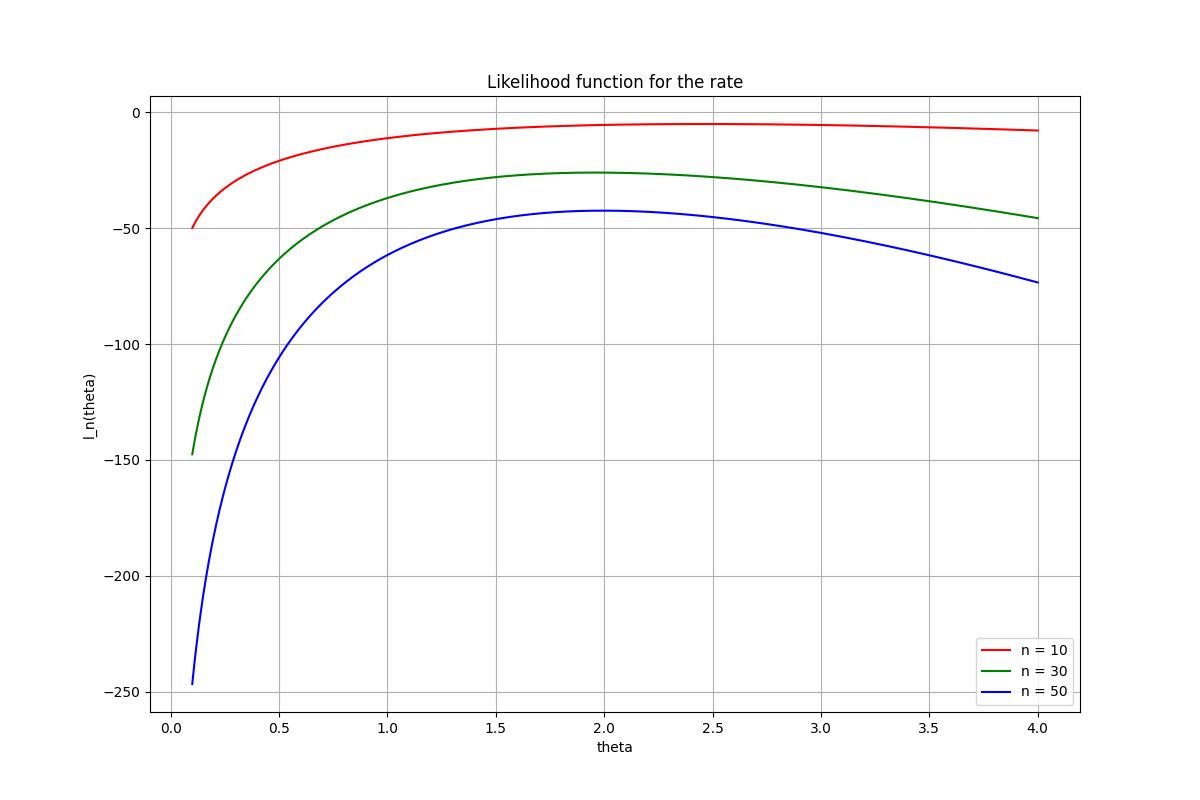
\includegraphics[width=1.0\linewidth]{images/gamma_likelihood.png}
    \caption{A graph of the likelihood function of \(\Gamma(2, \theta)\) for increasing samples.}
\end{figure}

Taking \(N = 200\) samples of size \(n = 10\) and \(n = 50\), we obtain \(x(1), \dots, x(N)\) independent random variables of size \(n\) from \(f(x \mid \theta)\) with corresponding maximum likelihood estimators \(\hat{\theta}_n(1), \dots, \hat{\theta}_n(N)\) of \(\theta\). Notice in the histogram plots for each case, the peaks are around \(2.2\) for both but the variance for \(n = 50\) is lower than that of \(n = 10\). 

Furthermore, given \(X_i \sim \Gamma(2, \theta)\), then \(\sum_{i=1}^n X_i \sim \Gamma(2n, \theta)\). This can be shown inductively by expressing \(X_i\) as the sum of two exponential random variables. Then \(\hat{\theta}_n = \frac{2n}{\sum_{i=1}^n x_i}\) follows an inverse Gamma distribution (equivalently, \(\hat{\theta}_n^{-1}\) is follows a Gamma distribution), which broadly matches the shape of our histogram. Moreover, this confirms that the variance should decrease as \(n\) increases.

\begin{figure}
    \centering
    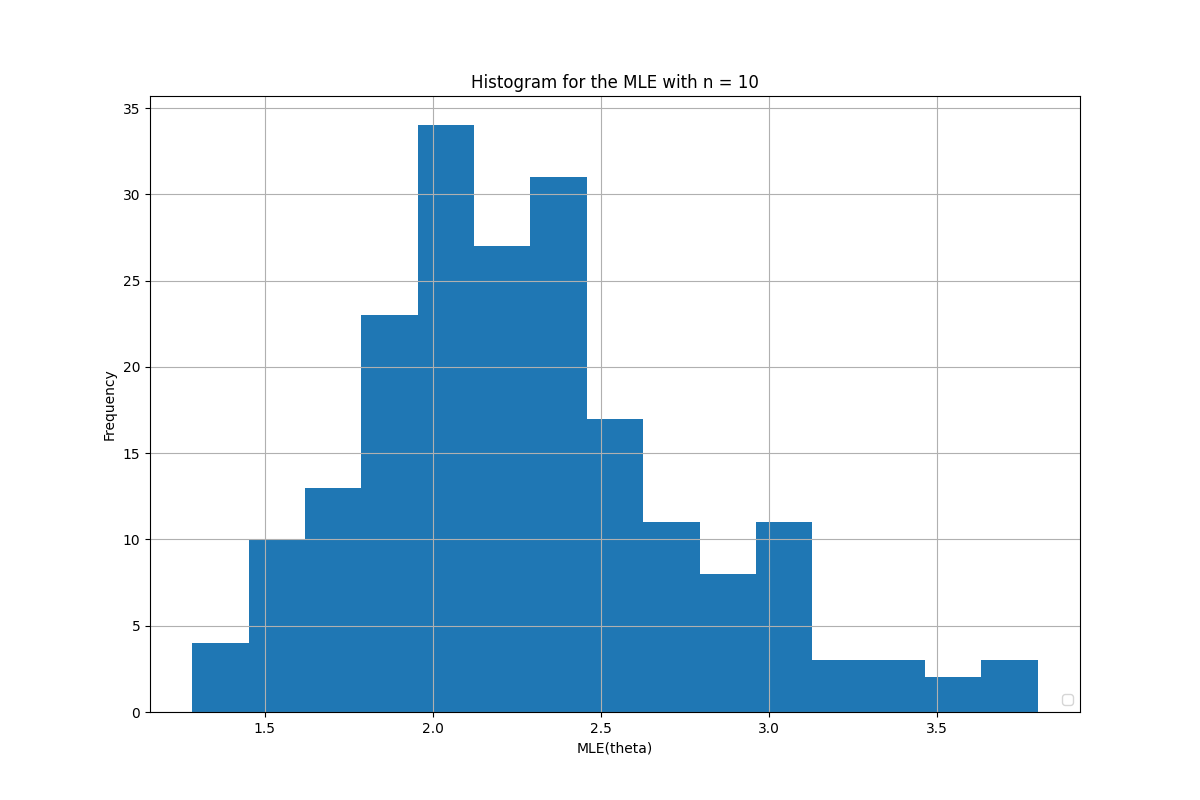
\includegraphics[width=0.49\linewidth]{images/gamma_hist_10.png}
    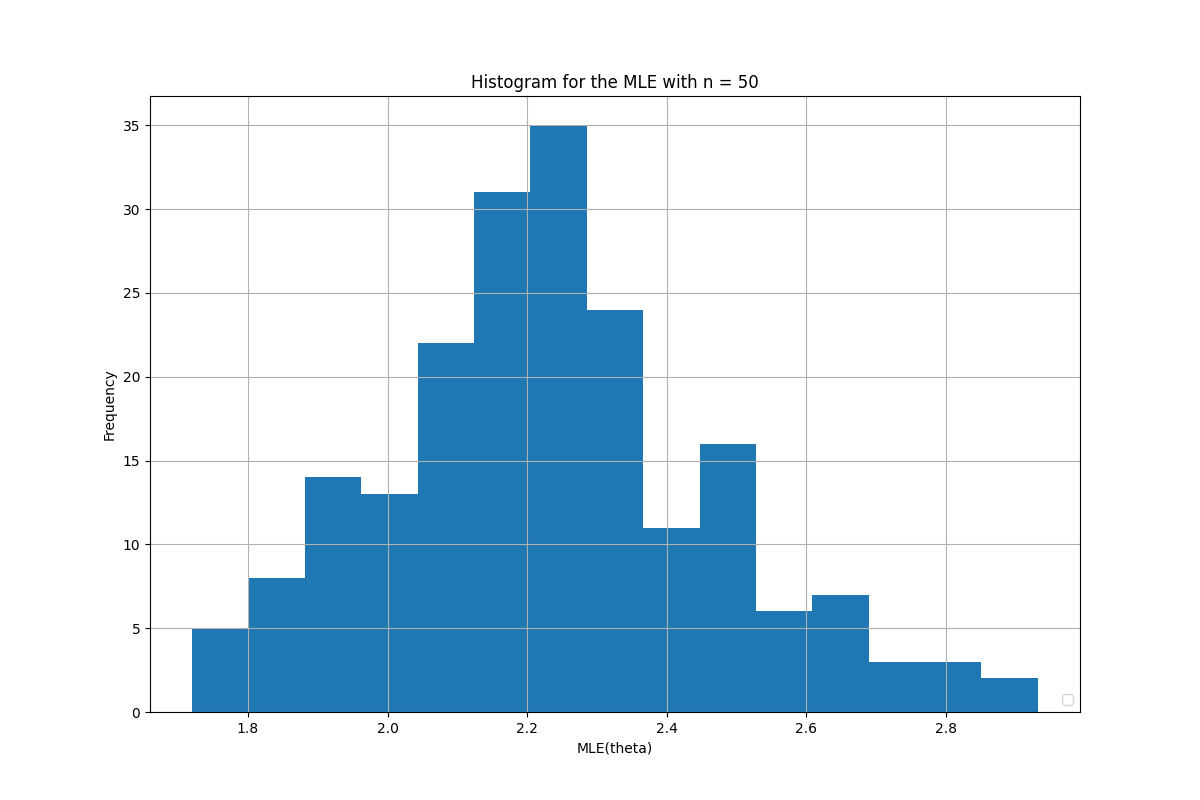
\includegraphics[width=0.49\linewidth]{images/gamma_hist_50.png}
    \caption{Histograms for the maximum likelihood estimate of \(\Gamma(2, 2.2)\) for \(200\) samples of size \(n = 10, 50\).}
\end{figure}

\section{Normal Distribution}

We want to generate a random sample \(X_1,\dots,X_n\) from \(N(\mu,\sigma^2)\) the normal distribution with mean \(\mu\) and variance \(\sigma^2\). Once again, we cannot use \(X = F^{-1}(U)\) where \(U \sim \mathop{\mathrm{Unif}}[0,1]\) and
\[ F(x) = \frac{1}{\sqrt{2\pi}}\int_{-\infty}^x \exp\left(-\frac{1}{2}v^2\right)\,dv, \]
since \(F^{-1}\) does not have a closed form. 

Instead, recall that if \((\Phi, V)\) have joint density function \(f(\phi, v)\) and we define
\[ X = X(\Phi, V), \quad Y = Y(\Phi, V), \]
such that \((X, Y)\) is an injective function of \((\Phi, V)\), then \((X, Y)\) has joint density function \(g(x, y)\) given by
\[ g(x, y) = f(\phi(x,y), v(x,y)) \left|\frac{\partial (\phi, v)}{\partial (x, y)}\right|. \]
Set
\[ f(\phi,v) = \frac{1}{4\pi}\exp\left(-\frac{v}{2}\right), \]
for \(0 \leq \phi \leq 2\pi\) and \(v \geq 0\). Define 
\[ X = \mu_1 + \sigma \sqrt{V} \cos\Phi, \quad Y = \mu_2 + \sigma\sqrt{V} \sin\Phi. \]
We compute the Jacobian of \((X, Y)\),
\[ \left|\frac{\partial (X, Y)}{\partial (V, \Phi)}\right| = \left| \matrix{\frac{\partial X}{\partial V} & \frac{\partial X}{\partial \Phi} \cr \frac{\partial Y}{\partial V} & \frac{\partial Y}{\partial \Phi} } \right| = \left| \matrix{ \frac{\sigma\cos\Phi}{2\sqrt V} & -\sigma\sqrt{V}\sin\Phi \cr \frac{\sigma\sin\Phi}{2\sqrt V} & -\sigma\sqrt{V}\cos\Phi } \right| = \frac{\sigma^2}{2}. \]
We also have \((x - \mu_1)^2 + (y - \mu_2)^2 = \sigma^2v\), therefore
\begin{eqnarray*}
    g(x, y) & = & f(\phi(x,y), v(x,y)) \left|\frac{\partial (V, \Phi)}{\partial (X, Y)}\right| \\
            & = & \frac{1}{2\pi\sigma^2}\exp\left(-\frac{(x-\mu_1)^2 + (y-\mu_2)^2}{2\sigma^2}\right) \\
            & = & \frac{1}{\sqrt{2\pi\sigma}}\exp\left(-\frac{(x-\mu_1)^2 }{2\sigma^2}\right)
                  \frac{1}{\sqrt{2\pi\sigma}}\exp\left(-\frac{(y-\mu_2)^2 }{2\sigma^2}\right),
\end{eqnarray*}
hence \(X \sim N(\mu_1, \sigma^2)\) and \(Y \sim N(\mu_2, \sigma^2)\) are independent by the factorisation criterion. We can generate a normal sample as follows:
\begin{enumerate}
    \item Generate \(A, B \sim \mathop{\mathrm{Unif}}[0,1]\) independent samples.
    \item Define \(\Phi = 2\pi A\) and \(V = -2\log(1-B)\).
    \item Set \(X = \mu + \sigma\sqrt{V}\cos\Phi\) and \(Y = \mu + \sigma\sqrt{V}\sin\Phi\)
\end{enumerate}
The following code implements this procedure with \(\sigma^2 = 1\) in Python:
\begin{minted}[autogobble, linenos]{python}
    def normal_sample(n, mu):
        A = np.random.uniform(0, 1, n)
        B = np.random.uniform(0, 1, n)
        Phi = (2 * np.pi) * A
        V = -2 * np.log(1 - B)
        X = mu + np.sqrt(V) * np.cos(Phi)
        Y = mu + np.sqrt(V) * np.sin(Phi)
        return X # Y is also normal
\end{minted}

To generate a \(100\gamma\%\)-confidence interval for \(\mu\), recall that \(\bar{X} \sim N(\mu, \frac{1}{n})\) by taking the expectation or variance of the sample mean. Let us normalise \(Z = \sqrt{n}(\bar{X} - \mu) \sim N(0,1)\) so that for \(z = \Phi^{-1}(\gamma)\), we have \(\pr(-z < Z < z) = \gamma\) if and only if 
\[ \pr\left(\bar{X} - \frac{z}{\sqrt{n}} < \mu < \bar{X} + \frac{z}{\sqrt{n}}\right) = \gamma. \]
Therefore,
\[ \left(\bar{X} - \frac{z}{\sqrt{n}}, \bar{X} + \frac{z}{\sqrt{n}}\right) \] 
is a \(100\gamma\%\)-confidence interval for \(\mu\).

Let \(\mu = 0\). We shall tabulate \(25\) samples of size \(n = 100\) and check whether the \(95\%\)-confidence interval contains \(\mu\).

\begin{verbatim}[Output]
    Mean        Lower       Upper       Contains?
    [-0.0525,   -0.2485,    0.1434,     1]
    [0.0572,    -0.1388,    0.2532,     1]
    [0.2125,    0.0165,     0.4085,     0]
    [-0.0435,   -0.2395,    0.1525,     1]
    [0.0633,    -0.1327,    0.2592,     1]
    [-0.1677,   -0.3637,    0.0283,     1]
    [-0.1157,   -0.3117,    0.0803,     1]
    [0.0598,    -0.1362,    0.2558,     1]
    [-0.0816,   -0.2776,    0.1144,     1]
    [0.1073,    -0.0887,    0.3033,     1]
    [-0.0239,   -0.2199,    0.1721,     1]
    [0.0963,    -0.0997,    0.2923,     1]
    [-0.0072,   -0.2032,    0.1888,     1]
    [-0.0546,   -0.2506,    0.1414,     1]
    [0.1375,    -0.0585,    0.3335,     1]
    [-0.0177,   -0.2137,    0.1783,     1]
    [-0.0203,   -0.2163,    0.1757,     1]
    [-0.0933,   -0.2893,    0.1027,     1]
    [-0.0247,   -0.2207,    0.1713,     1]
    [0.1194,    -0.0765,    0.3154,     1]
    [-0.0881,   -0.2841,    0.1079,     1]
    [-0.2185,   -0.4145,    -0.0225,    0]
    [0.0711,    -0.1249,    0.2671,     1]
    [0.0516,    -0.1444,    0.2476,     1]
    [-0.0733,   -0.2693,    0.1227,     1]
\end{verbatim}
In this experiment, there were only \(2\) out of \(25\) times that the confidence interval did not contain the mean \(\mu = 0\), which is close to \(95\%\). This is expected, since a \(95\%\)-confidence interval has probability \(0.95\) of containing the mean. Let \(B\) be the number of times the mean lies in the \(95\%\)-confidence interval. By independence, \(B \sim \mathop{\mathrm{Binom}}(0.95,25)\), with expectation \(0.95 \cdot 25 = 23.75\). 

If we were to repeat this experiment with lower \(n = 50\), then the distribution of \(B\) and therefore the expectation that the mean lies in the \(95\%\)-confidence interval remains the same. This is also owing to the fact that decreasing \(n\) will increase the width of the confidence interval.

\section{\(\chi^2\) Distribution}

By definition, for \(Z_1, \dots Z_k \sim N(0,1)\) independent standard normal distributions, the sum of their squares \(X = \sum_{i=1}^k Z^2_i\) has a \(\chi^2\) distribution with \(k\) degrees of freedom. The following program generates a \(\chi^2_k\) sample of size \(n\):

\begin{minted}[autogobble, linenos]{python}
    def chi_square_sample(n, k):
        Z = normal_sample((n, k), 0) 
        x = np.sum(np.square(Z), axis=1)
        return x
\end{minted}

As we increase \(n\), we expect the histogram is match the probability density function more closely. As \(k\) increases, the mean \(k\) increases, the variance \(2k\) increases but the skewness \(\sqrt{8/k}\) decreases. All these features are reflected in our histogram plots where we take \(n = 500\) and \(k = 1, 3, 5, 40\).

\begin{figure}
    \centering
    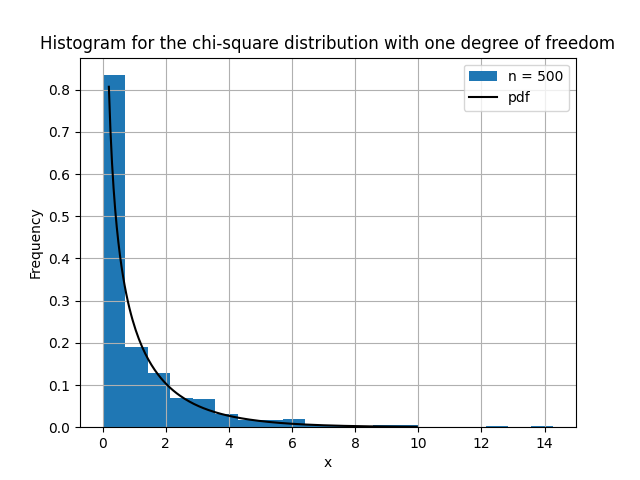
\includegraphics[width=0.49\linewidth]{images/chi_square_500_1.png}
    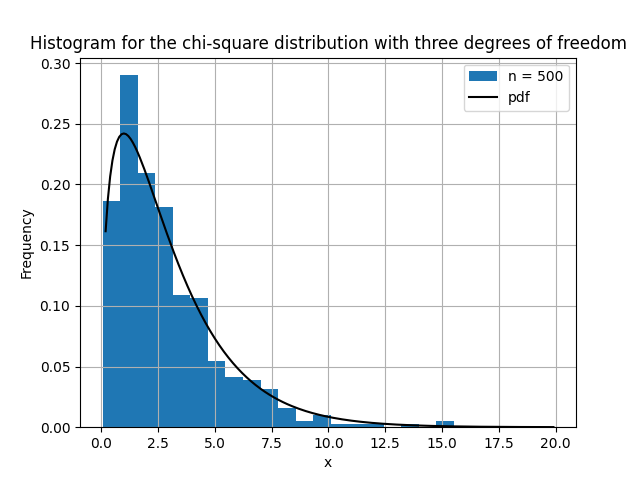
\includegraphics[width=0.49\linewidth]{images/chi_square_500_3.png}
    \caption{Histograms of \(\chi^2_k\) samples superimposed with the probability density function of the \(\chi^2_k\) distribution with \(k = 1, 3\) degrees of freedom.}
\end{figure}

\begin{figure}
    \centering
    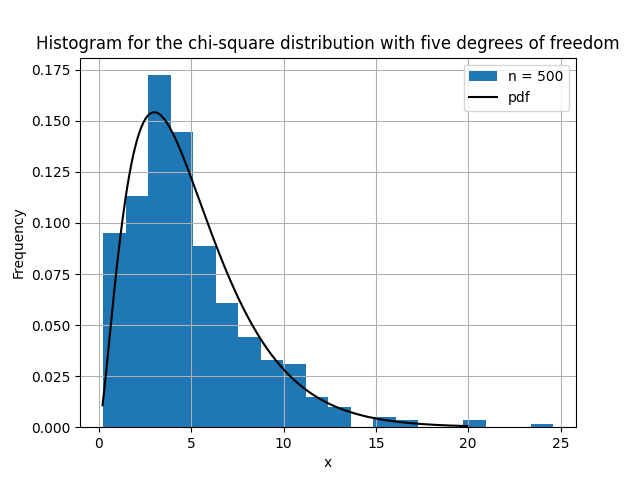
\includegraphics[width=0.49\linewidth]{images/chi_square_500_5.png}
    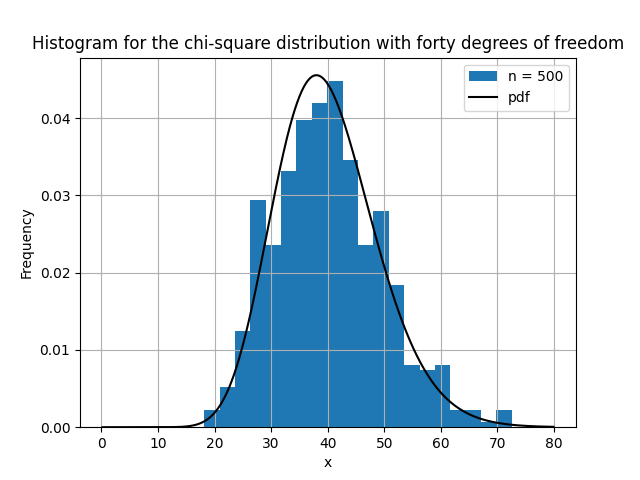
\includegraphics[width=0.49\linewidth]{images/chi_square_500_40.png}
    \caption{Histograms of \(\chi^2_k\) samples superimposed with the probability density function of the \(\chi^2_k\) distribution with \(k = 5, 40\) degrees of freedom.}
\end{figure}

Similarly, we could plot other related useful distributions, such as the \(F\)-distribution which is a ratio of two \(\chi^2\) distributions, the Student-\(t\) distributions which is a ratio of a normal distribution with the square root of a \(\chi^2\) distribution.

\section{Statistics in Python}

Python (along with R) is one of the main languages used for statistics, data analysis and machine learning. Libraries such as NumPy, SciPy, MatPlotLib and Pandas are heavily used to deal with data, whilst libraries such as PyTorch, TensorFlow and Scikit-Learn are increasing used to perform statistical learning techniques such as classification of categorical data, regression of quantitative data, clustering of unlabelled data and dimensionality reduction.

An ubiquitous technique in statistics is least squares regression which plots the best line of fit by minimising the sum of the squared residuals. This can be implemented in SciPy and NumPy through the optimize.curve\_fit and linalg.lstsq functions. 

\begin{minted}[autogobble, linenos]{python}
    import numpy as np
    from scipy import optimize
    
    x = np.linspace(0, 1, 101)
    y = 1 + x + x * np.random.random(len(x))
    A = np.vstack([x, np.ones(len(x))]).T
    y = y[:, np.newaxis]

    # Direct inverse method
    alpha = np.dot((np.dot(np.linalg.inv(np.dot(A.T,A)),A.T)),y)

    # Pseudo-inverse method
    pinv = np.linalg.pinv(A)
    alpha = pinv.dot(y)

    # Least squares in NumPy
    alpha = np.linalg.lstsq(A, y, rcond=None)[0]

    # Optimise curve from SciPy
    def func(x, a, b):
        y = a*x + b
        return y
    alpha = optimize.curve_fit(func, xdata = x, ydata = y)[0]
\end{minted}
\end{document}
